% Privacy-first section 7: what a practitioner can do, and why the usual metric will not help.
% Budget 1.25 pages including Table~\ref{tab:blind} and Figure~\ref{fig:blind}.
% Early stopping: outputs/nt_{ckpt,seeds}/nt250m_mlm_ecoli_s*, ep3/ep15/ep50, one basis 19 Oct.
% Blind metric: outputs/nt_ckpt/nt250m_mlm_human_s0/utility_at_leak.json and bpe_human/*, 19-20 Oct.
\section{What a practitioner can do, and what will not warn them}
\label{sec:blind}

Two of the results above have an operational reading. Stopping where held-out loss stops improving
does prevent capture, but the margin is three hundredths of a bit, and the number practitioners
actually select on cannot resolve it.

\paragraph{At the optimum there is nothing to extract, because nothing is stored yet.}
It is worth distinguishing a record that is hidden from one that is absent. At the best saved
checkpoint of Nucleotide Transformer on \emph{E.~coli}, the leave-one-out probe, with every other
target nucleotide supplied and one masked, reads $0.01$, exactly the never-trained control, and the
planted
record's surprise is $2.128$ and $2.115$\,\bits{} against $2.110$ for a matched non-member. The
member is indistinguishable from a non-member on the model's own scale. No decoder can recover what
is not there, and our strongest decoder recovers 0\%.

Three hundredths of a bit later this is no longer true: across three seeds, 8\%, 8\% and 14\% of
records come back whole. Further out, at +0.44\,\bits, 66--76\%. The defence is real and the
transition is abrupt. Our own from-scratch backbone tolerates roughly ten times that drift before
leaking at all, so a study run only on a model one trains oneself reads more reassuringly than
released weights warrant. That is why this paper is built on released weights.

\paragraph{The number people select on moves by one per cent.}
Nobody chooses a genomic checkpoint by held-out loss. They choose by downstream task score.
Table~\ref{tab:blind} puts that score beside the leak at every checkpoint of the same runs.

\begin{table}[t]
\centering
\caption{Downstream task score measured at every checkpoint, beside the leak from the same weights.
GUE promoter classification, linear probe on frozen mean-pooled states, Matthews correlation on the
full held-out split. \emph{id} is single-copy identification as in \S\ref{sec:ident}.}
\label{tab:blind}
\begin{tabular}{llcccc}
\toprule
model & checkpoint & held-out \bits & MCC & 16-copy verbatim & 1-copy id \\
\midrule
NT 250M, chr22 & round 15 (best MCC) & 1.411 & \textbf{0.802} & \textbf{6\%}  & \textbf{0.04} \\
               & round 30            & 1.501 & 0.798          & 12\%          & 0.17 \\
               & round 50            & 1.632 & 0.780          & 18\%          & 0.35 \\
\midrule
DNABERT-2, chr22 & round 15 (best MCC) & 1.264 & 0.798--0.801 & 0\%   & 0.00 \\
                 & round 120           & 1.600 & 0.784--0.792 & 30--50\% & 0.70--0.80 \\
                 & final               & 1.729 & 0.782--0.787 & 40--44\% & 0.92--0.96 \\
\bottomrule
\end{tabular}
\end{table}

On DNABERT-2 the score declines across the run by 1.1--1.6 points of MCC in total, monotonically in
two seeds and with one reversal at round~50 in the third, while single-copy identification climbs
from nothing to 0.92--0.96 (Figure~\ref{fig:blind}). Selecting on that score
would pick round~15, which is also the safe checkpoint, so the metric is not misleading there. It
carries no information either: a practitioner watching it sees a flat line through the entire
interval in which the model learns to identify individuals.

On NT fine-tuned on chromosome~22 the situation is worse, because there is no clean checkpoint for
the metric to point at. The highest task score belongs to the earliest checkpoint saved, and that one
already reproduces 6\% of repeated records and identifies 4\% of single copies. Choosing the best
available model by downstream performance means choosing a model that is already leaking.

\begin{figure}[t]
\centering
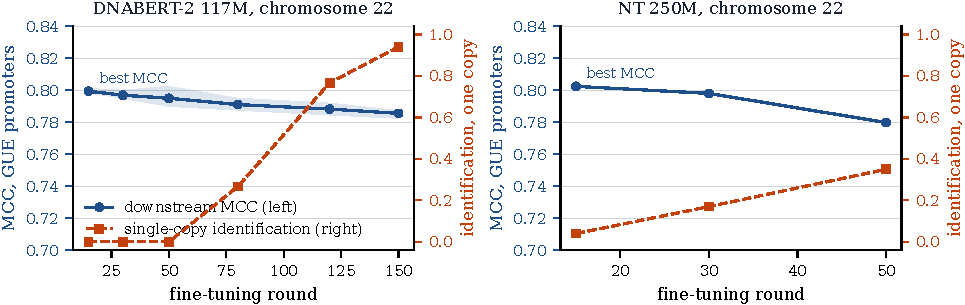
\includegraphics[width=\linewidth]{F7_blind.pdf}
\caption{Downstream score and leak, measured on the same weights at the same checkpoints.
\textbf{Left:} DNABERT-2 on chromosome~22, three seeds, band over seeds. The score falls by
1.1--1.6 points of MCC across a run in which single-copy identification goes from zero to 0.94.
\textbf{Right:} Nucleotide Transformer 250M on the same corpus, where the best downstream score is
the earliest checkpoint saved and that checkpoint already identifies 4\% of single copies. Linear
probe on frozen mean-pooled states, GUE promoter classification, full held-out split.}
\label{fig:blind}
\end{figure}


\paragraph{Recommendation.}
Three things follow, and we state them as the guidance we would give rather than as results.

\emph{Stop where held-out loss stops improving, and compute it.} It is the only quantity we measured
that moves before the leak does, and in a fine-tuning pipeline it is nearly free.

\emph{Do not treat downstream score as a safety signal.} Across six tasks and two organisms it never
moved more than one to two per cent while extraction went to saturation. It is evidence about
utility and nothing else.

\emph{Prefer a tokenizer with more slots, and measure what it costs you.} A model whose canary spans
24 or 48 token positions did not leak at any loss we drove it to, including losses far past
usefulness. That is the strongest protective effect we found. It is not free: fine-grained
tokenizers carry their own costs in sequence length and downstream accuracy, which are
task-dependent and which we did not measure across the board. We therefore offer the slot count as a
lever worth pricing rather than a setting we can recommend blind.
